\chapter{Лабораторная работа 4 \\
Проектирование балансного смесителя на диодах}

Цель работы: получить навыки проектирования балансного смесителя на диодах в среде моделирования Advanced Design System (ADS).

\section{Техническое задание}

Спроектировать балансный смеситель на диодах HSMS-8101.
В качестве подложки использовать RO3003 с диэлектрической проницаемостью $\epsilon = 3.0$, толщиной диэлектрика $H = 0.5~\text{мм}$ и толщиной металлизации $t = 0.017~\text{мм}$.
Частотные параметры: $f_{RF} = 9.8~\text{ГГц}$, $f_{IF} = 1.1~\text{ГГц}$, $\Delta f_{-3dB} = 150~\text{МГц}$.

\section{Выполнение работы}

\subsection{Проектирование балансного смесителя на диодах}

\subsubsection{Расчёт кольцевого НО}

С помощью умного компонента \elementname{RRCoupler} из палитры \elementname{Passive Circuit DG --- Microstrip Circuits} спроектируем кольцевой делитель.
Для этого создадим временную схему (Рис.~\ref{fig:balanced_mixer_schematic_1}) и по команде Design в окне Design Guide/Passive Circuit \textrightarrow\ Passive Circuit Control Window.

\begin{figure}[!ht]
    \centering
    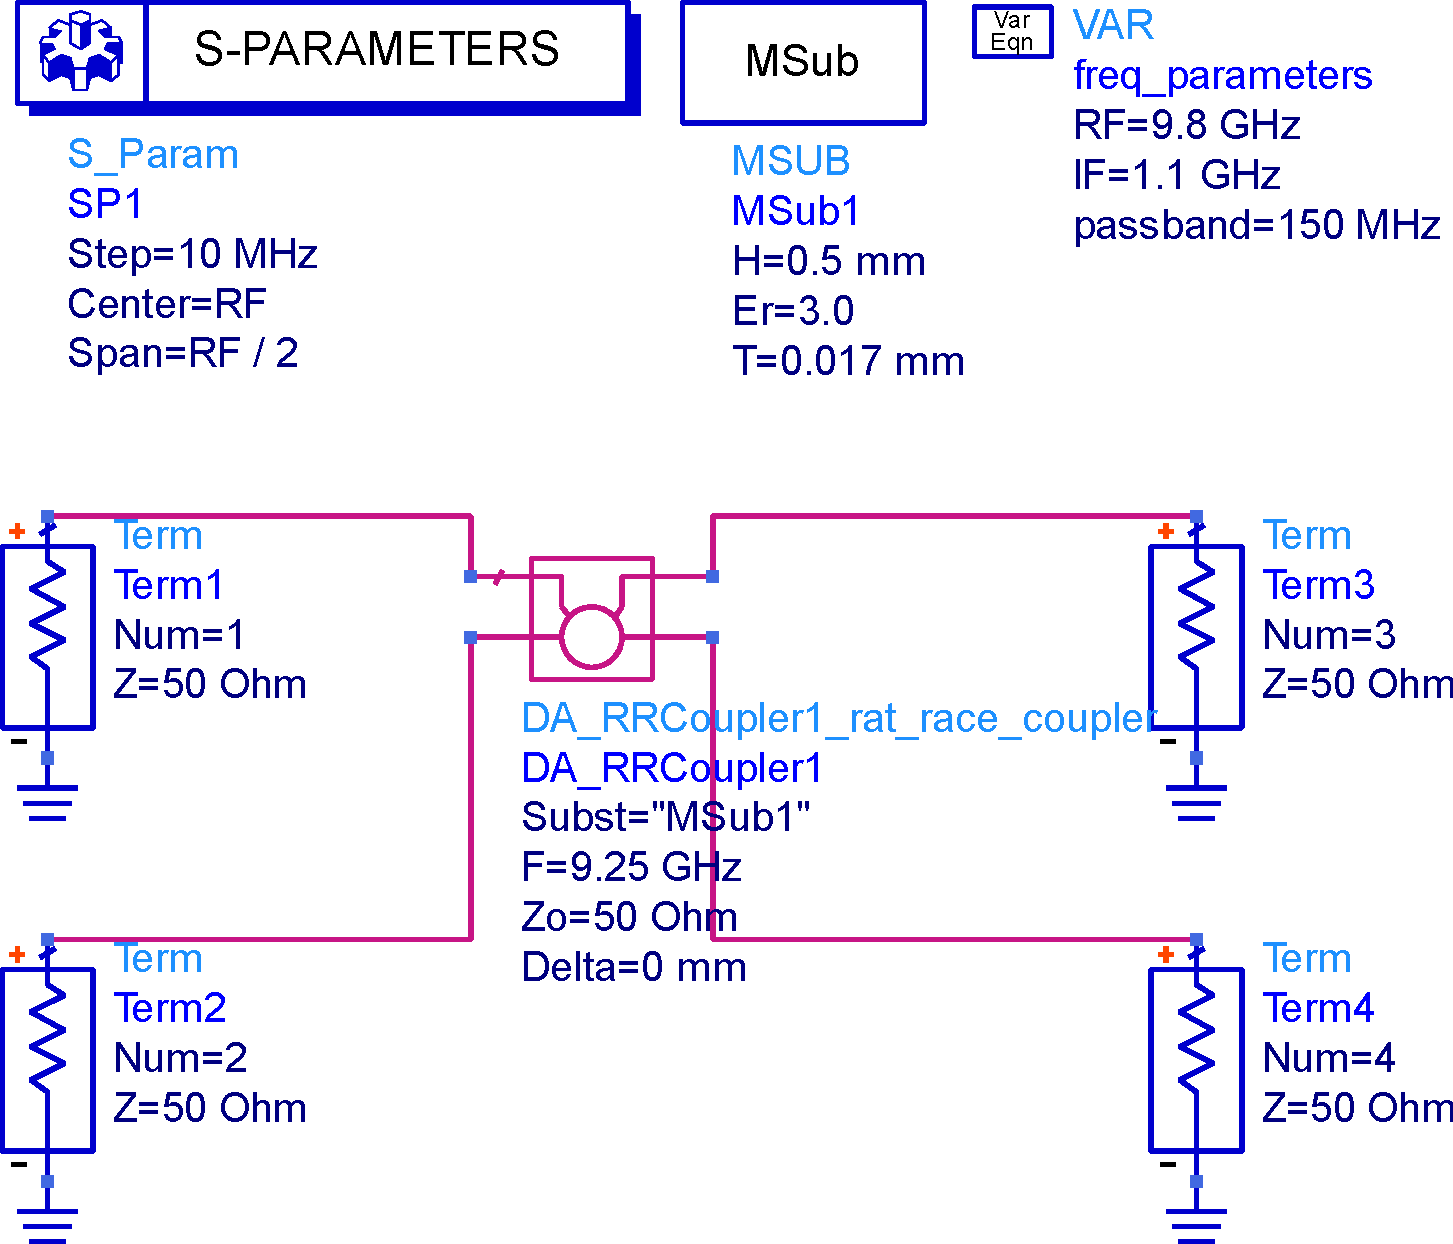
\includegraphics[width=0.6\textwidth]{balanced_mixer_schematic_1.pdf}
    \caption{Схема для синтеза кольцевого развязанного делителя}%
    \label{fig:balanced_mixer_schematic_1}
\end{figure}

Промоделируем её и выведем в окне данных АЧХ и ФЧХ моделируемого компонента (Рис.~\ref{fig:balanced_mixer_data_1}).

\begin{figure}[!ht]
    \centering
    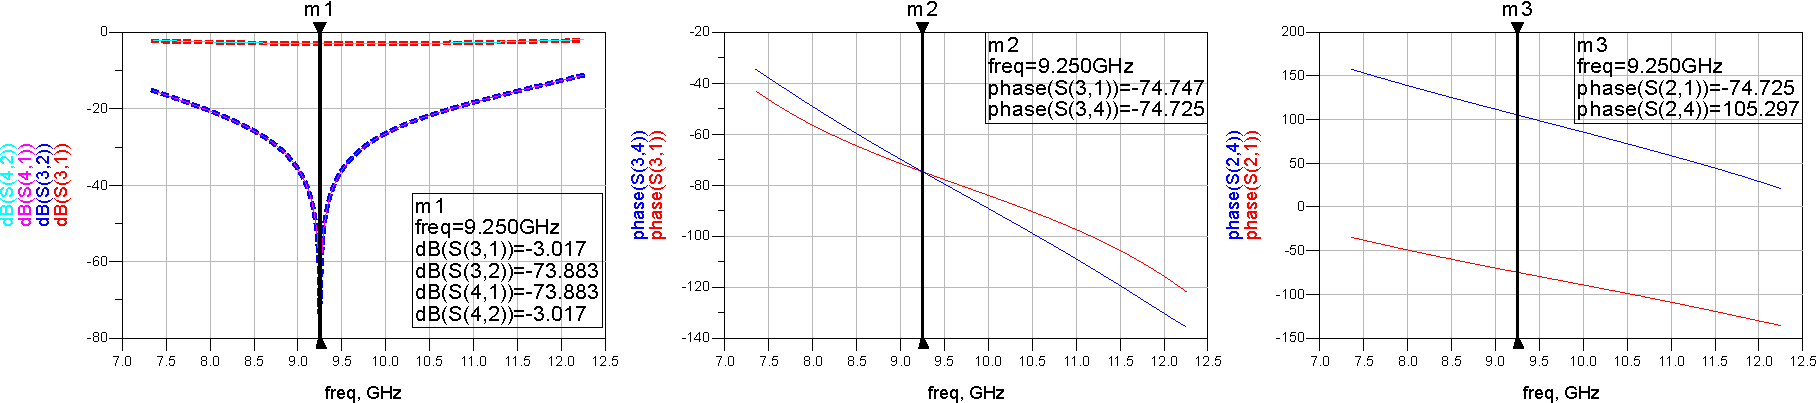
\includegraphics[width=\textwidth]{balanced_mixer_data_1.pdf}
    \caption{%
        (а) АЧХ кольцевого развязанного делителя;
        (б) ФЧХ кольцевого развязанного делителя по второму выходу;
        (в) ФЧХ кольцевого развязанного делителя по третьему выходу;
    }%
    \label{fig:balanced_mixer_data_1}
\end{figure}

\subsubsection{Проектирование короткозамкнутых шлейфов}

С помощью инструмента LineCalc выполним расчёт геометрических размеров микрополосковых линий.
Установим параметры подложки и рассчитаем длину $90^\circ$ на средней для RF и LO частоте, после чего установим минимальную для выбранного технологического процесса ширину в $0.2~\text{мм}$.
Получим значения $W = 0.2~\text{мм}$, $L = 5.19~\text{мм}$.

\subsubsection{Расчёт согласующих цепей диодной сборки}

Спроектируем согласующие цепи диодной сборки для частоты ВЧ (средняя для RF и LO).
Запустим моделирования и выведем на экране данных диаграмму Смита, на которой отобразим зависимость $S_{11}$ и $S_{22}$ от входной мощности (Рис.~\ref{fig:balanced_mixer_data_2_smith_1}) и окружность, соответствующую $\text{КСВН } = 1.5$.
Линии смещены вниз вправо.
Выберем на них какую-то точку близкую к середине и возьмём соответствующее ей значение импеданса, после чего внесём его в качестве параметра $Z_\text{load}$ умного компонента \elementname{DA\_SSMatch}.
Работа с этим элементом аналогична работе с элементом \elementname{RRCoupler}.
В результате долгого и кропотливого подбора импеданса получим результат как на Рис.~\ref{fig:balanced_mixer_data_2_smith_2}, которому соответствует схема на Рис.~\ref{fig:balanced_mixer_schematic_2}.

\begin{figure}[!ht]
    \centering
    \begin{subfigure}[b]{0.45\textwidth}
        \centering
        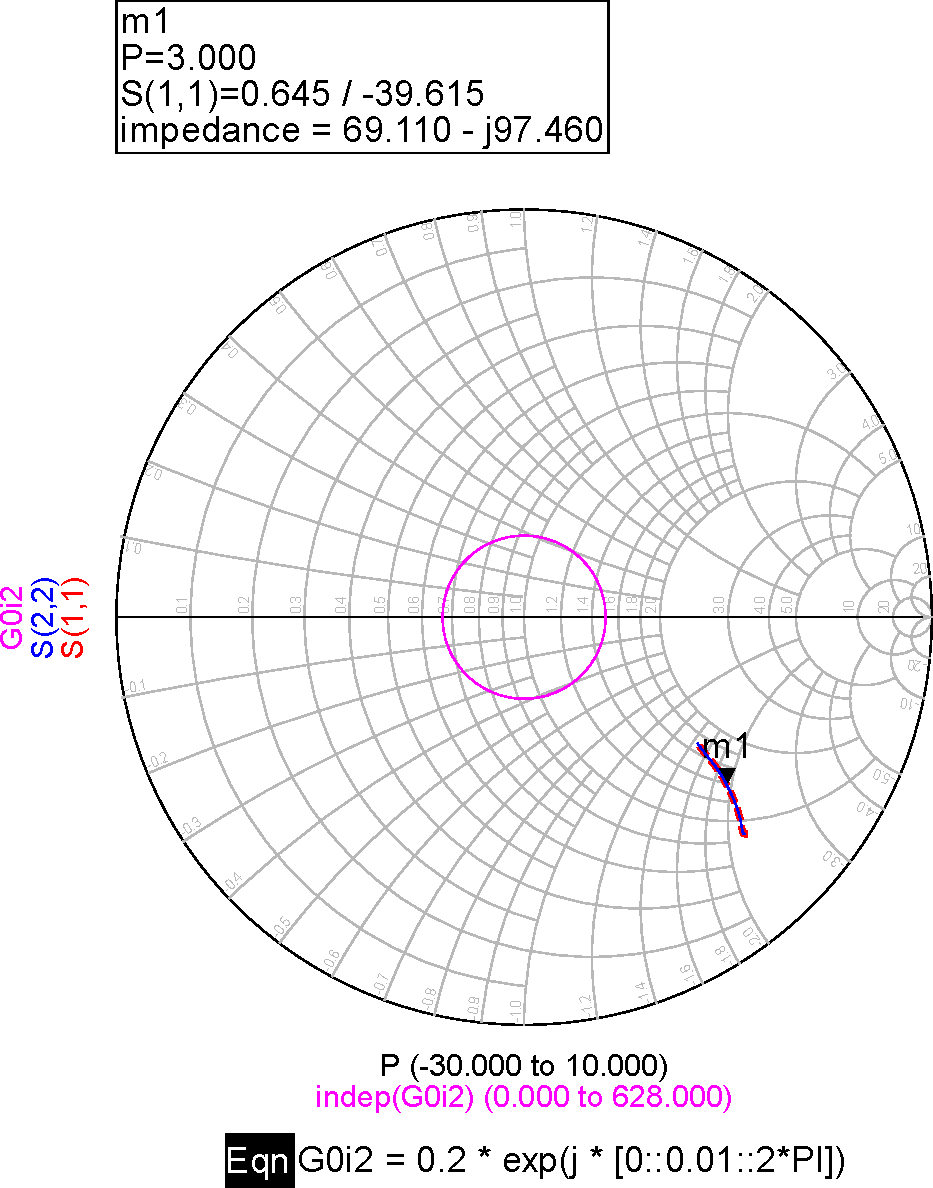
\includegraphics[width=\textwidth]{balanced_mixer_data_2_smith_1.pdf}
        \caption{}%
        \label{fig:balanced_mixer_data_2_smith_1}
    \end{subfigure}
    \hfill
    \begin{subfigure}[b]{0.45\textwidth}
        \centering
        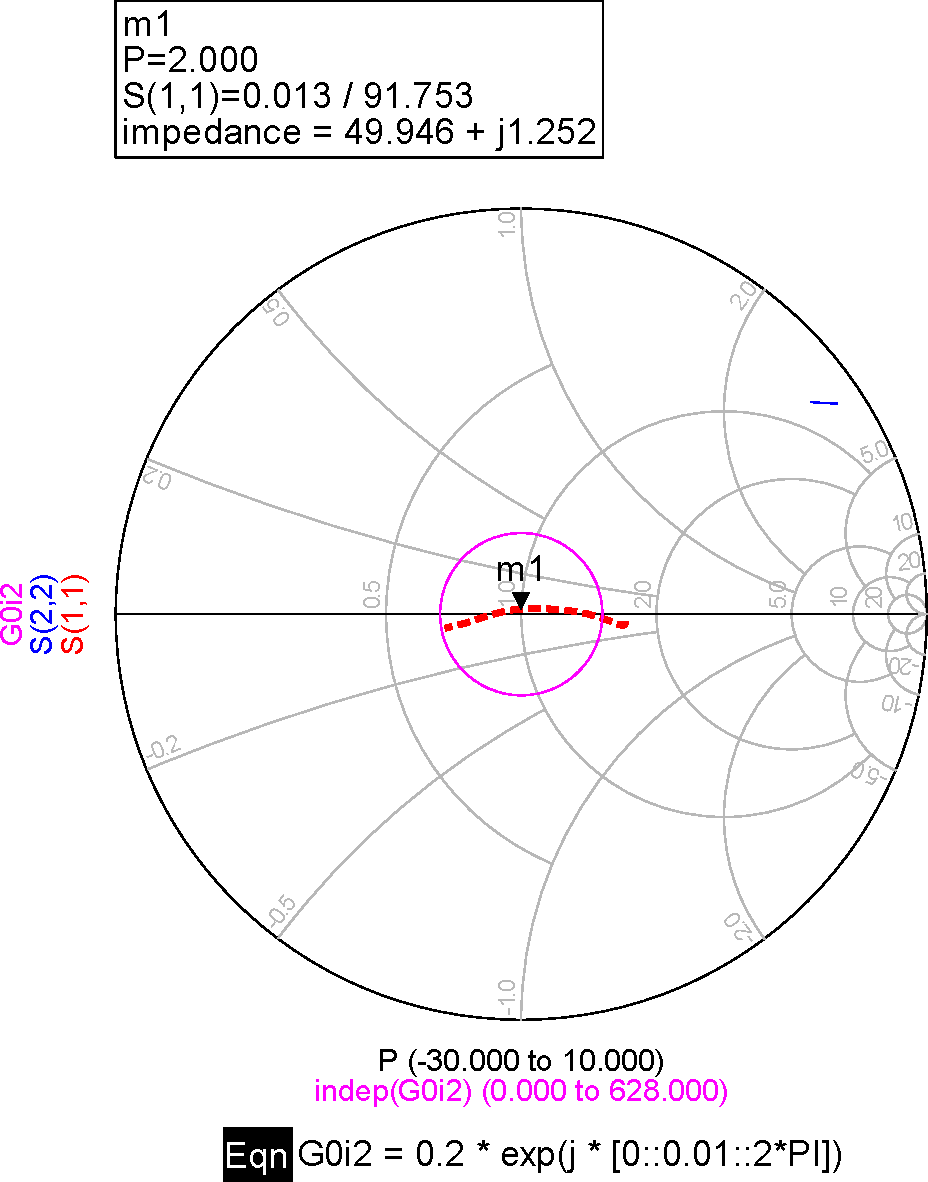
\includegraphics[width=\textwidth]{balanced_mixer_data_2_smith_2.pdf}
        \caption{}%
        \label{fig:balanced_mixer_data_2_smith_2}
    \end{subfigure}
    \caption{%
    }%
    \label{fig:balanced_mixer_data_2}
\end{figure}

\begin{figure}[!ht]
    \centering
    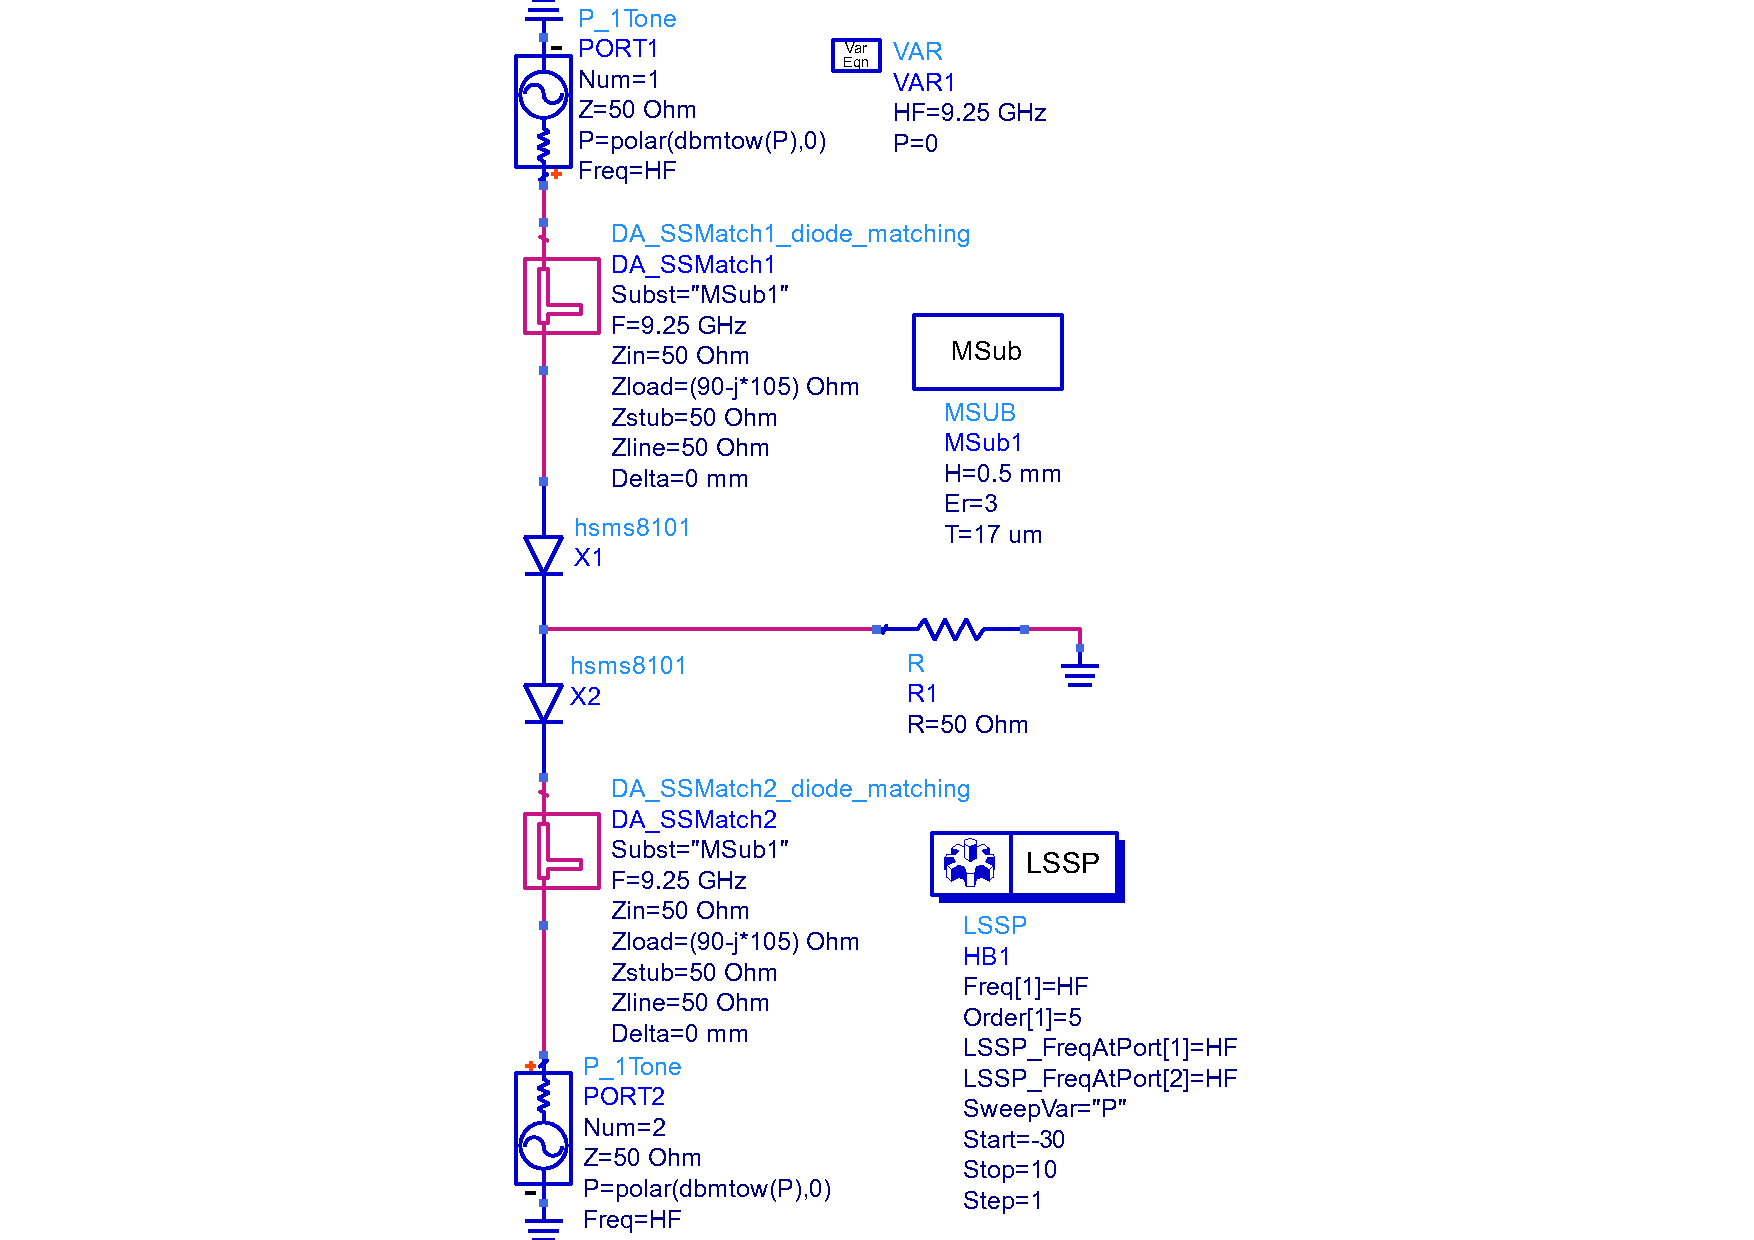
\includegraphics[width = 0.4\textwidth]{balanced_mixer_schematic_2.pdf}
    \caption{}%
    \label{fig:balanced_mixer_schematic_2}
\end{figure}

\subsubsection{Проектирование широкополосного шлейфа <<бабочка>>}

Аналогичным образом синтезируем широкополосный шлейф <<бабочка>>.
Схема представлена на Рис.~\ref{fig:balanced_mixer_schematic_3} а результаты моделирования на Рис.~\ref{fig:balanced_mixer_data_3_freq_response}.

\begin{figure}[!ht]
    \centering
    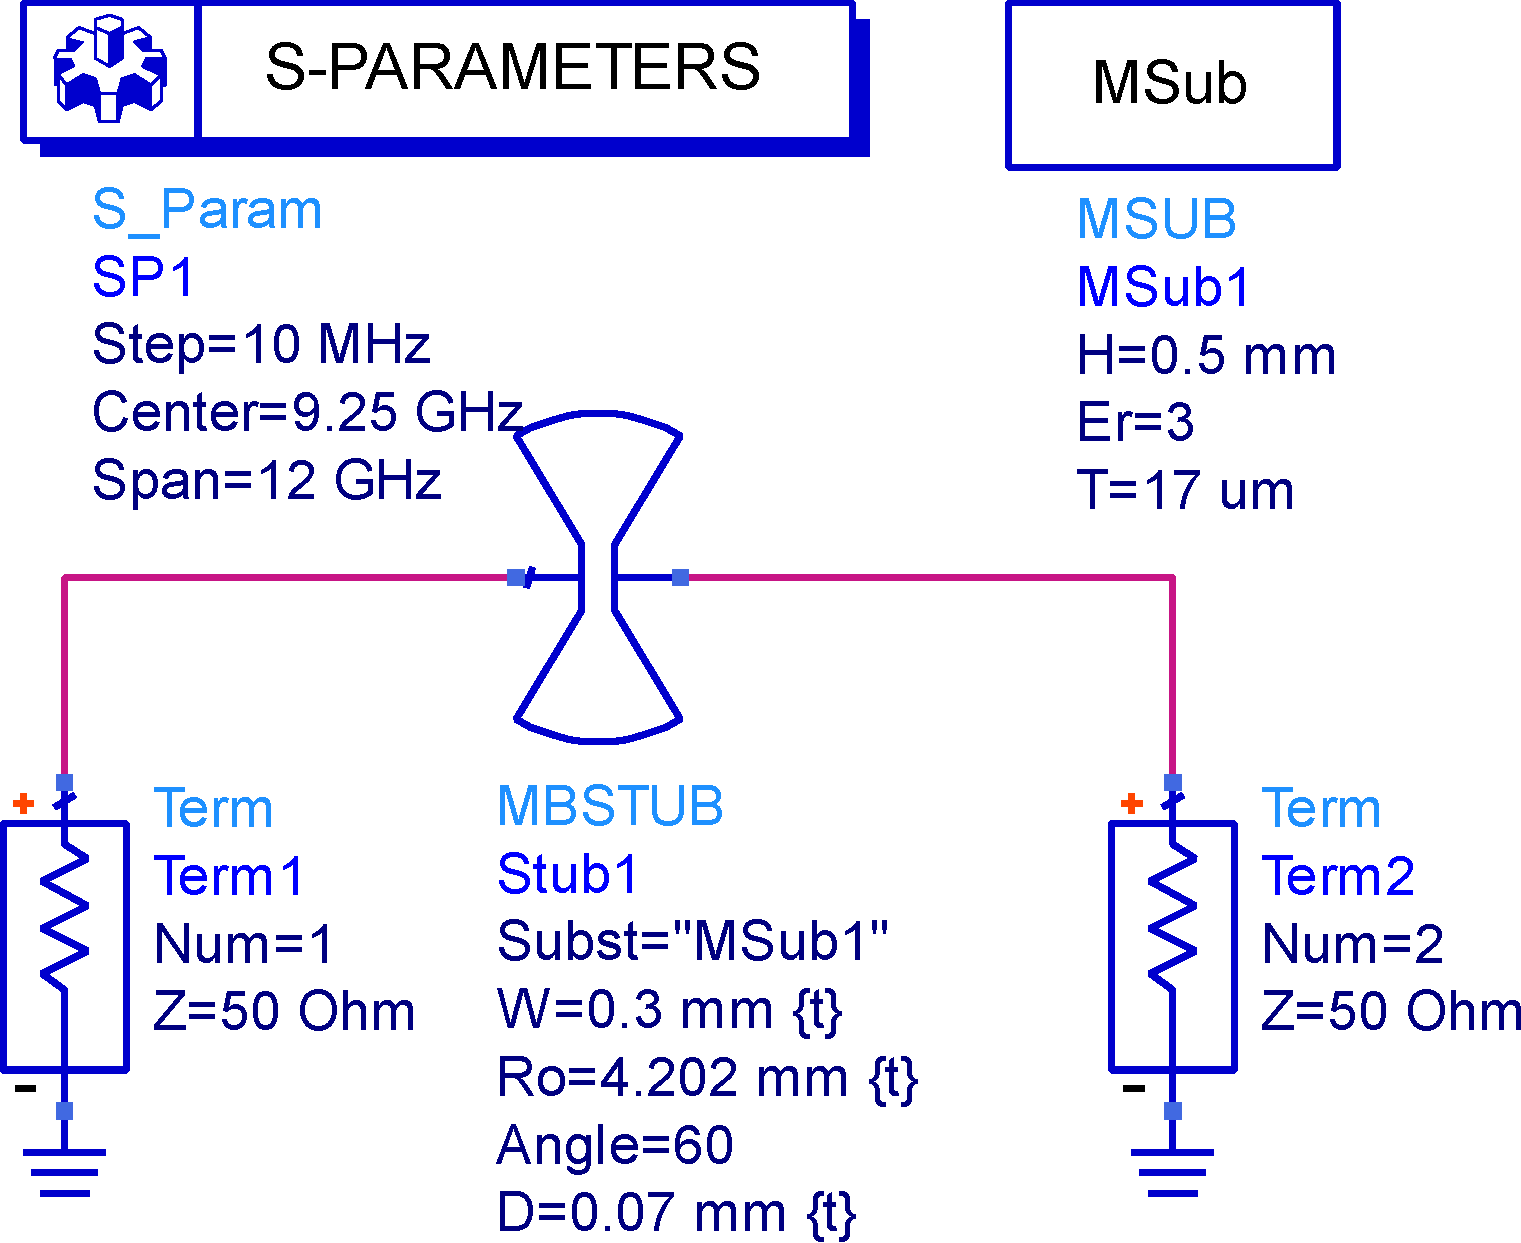
\includegraphics[width=0.8\textwidth]{balanced_mixer_schematic_3.pdf}
    \caption{}%
    \label{fig:balanced_mixer_schematic_3}
\end{figure}

\begin{figure}[!ht]
    \centering
    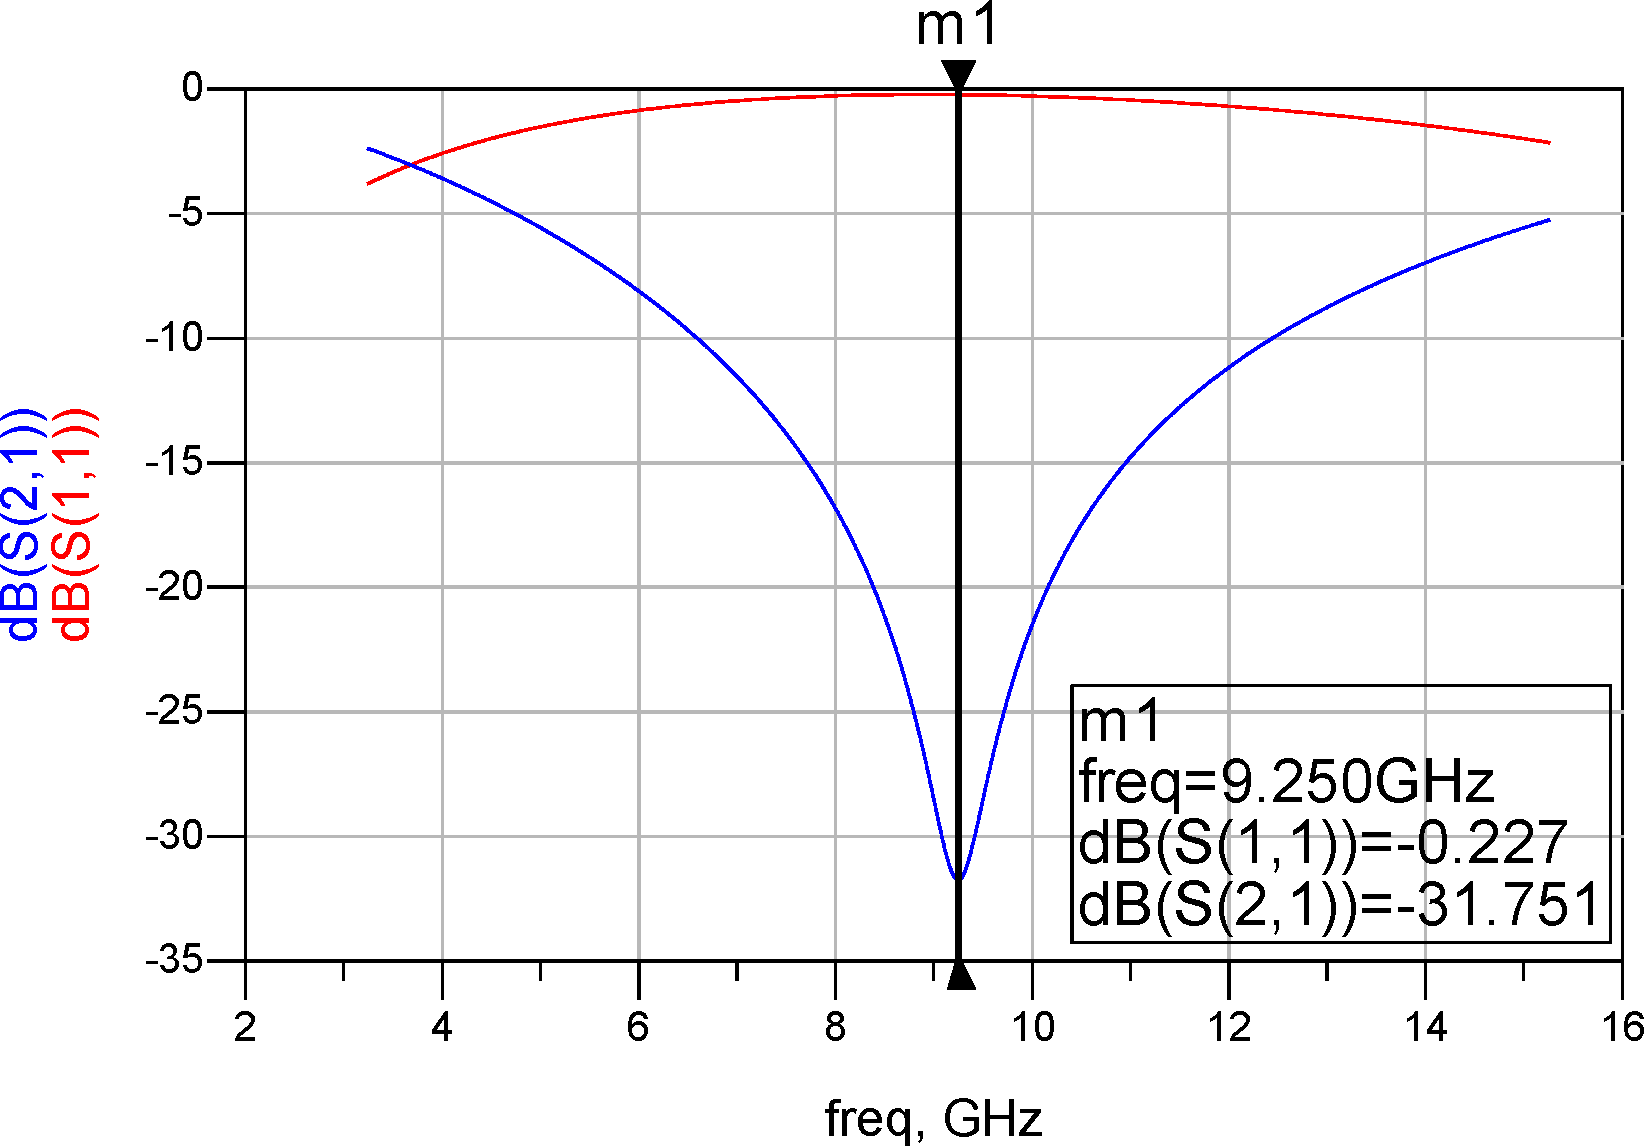
\includegraphics[width=0.6\textwidth]{balanced_mixer_data_3_freq_response.pdf}
    \caption{}%
    \label{fig:balanced_mixer_data_3_freq_response}
\end{figure}

\subsubsection{Проектирование ФНЧ}

Аналогичным образом выполним синтез ФНЧ.
Для этого соберём схему на Рис.~\ref{fig:balanced_mixer_schematic_6}.
Параметры синтеза можно увидеть на Рис.~\ref{fig:balanced_mixer_filter_design}
В результате синтеза внутенняя схема приобретёт вид как на Рис.~\ref{fig:balanced_mixer_schematic_4}.
Округлим номиналы компонентов до соответствия с стандартизированным рядом номиналов (Рис.~\ref{fig:balanced_mixer_schematic_5}).
Запустим моделирование и выведем АЧХ фильтра (Рис.~\ref{fig:balanced_mixer_data_4_freq_response}) отметив маркером интересующие точки.

\begin{figure}[!ht]
    \centering
    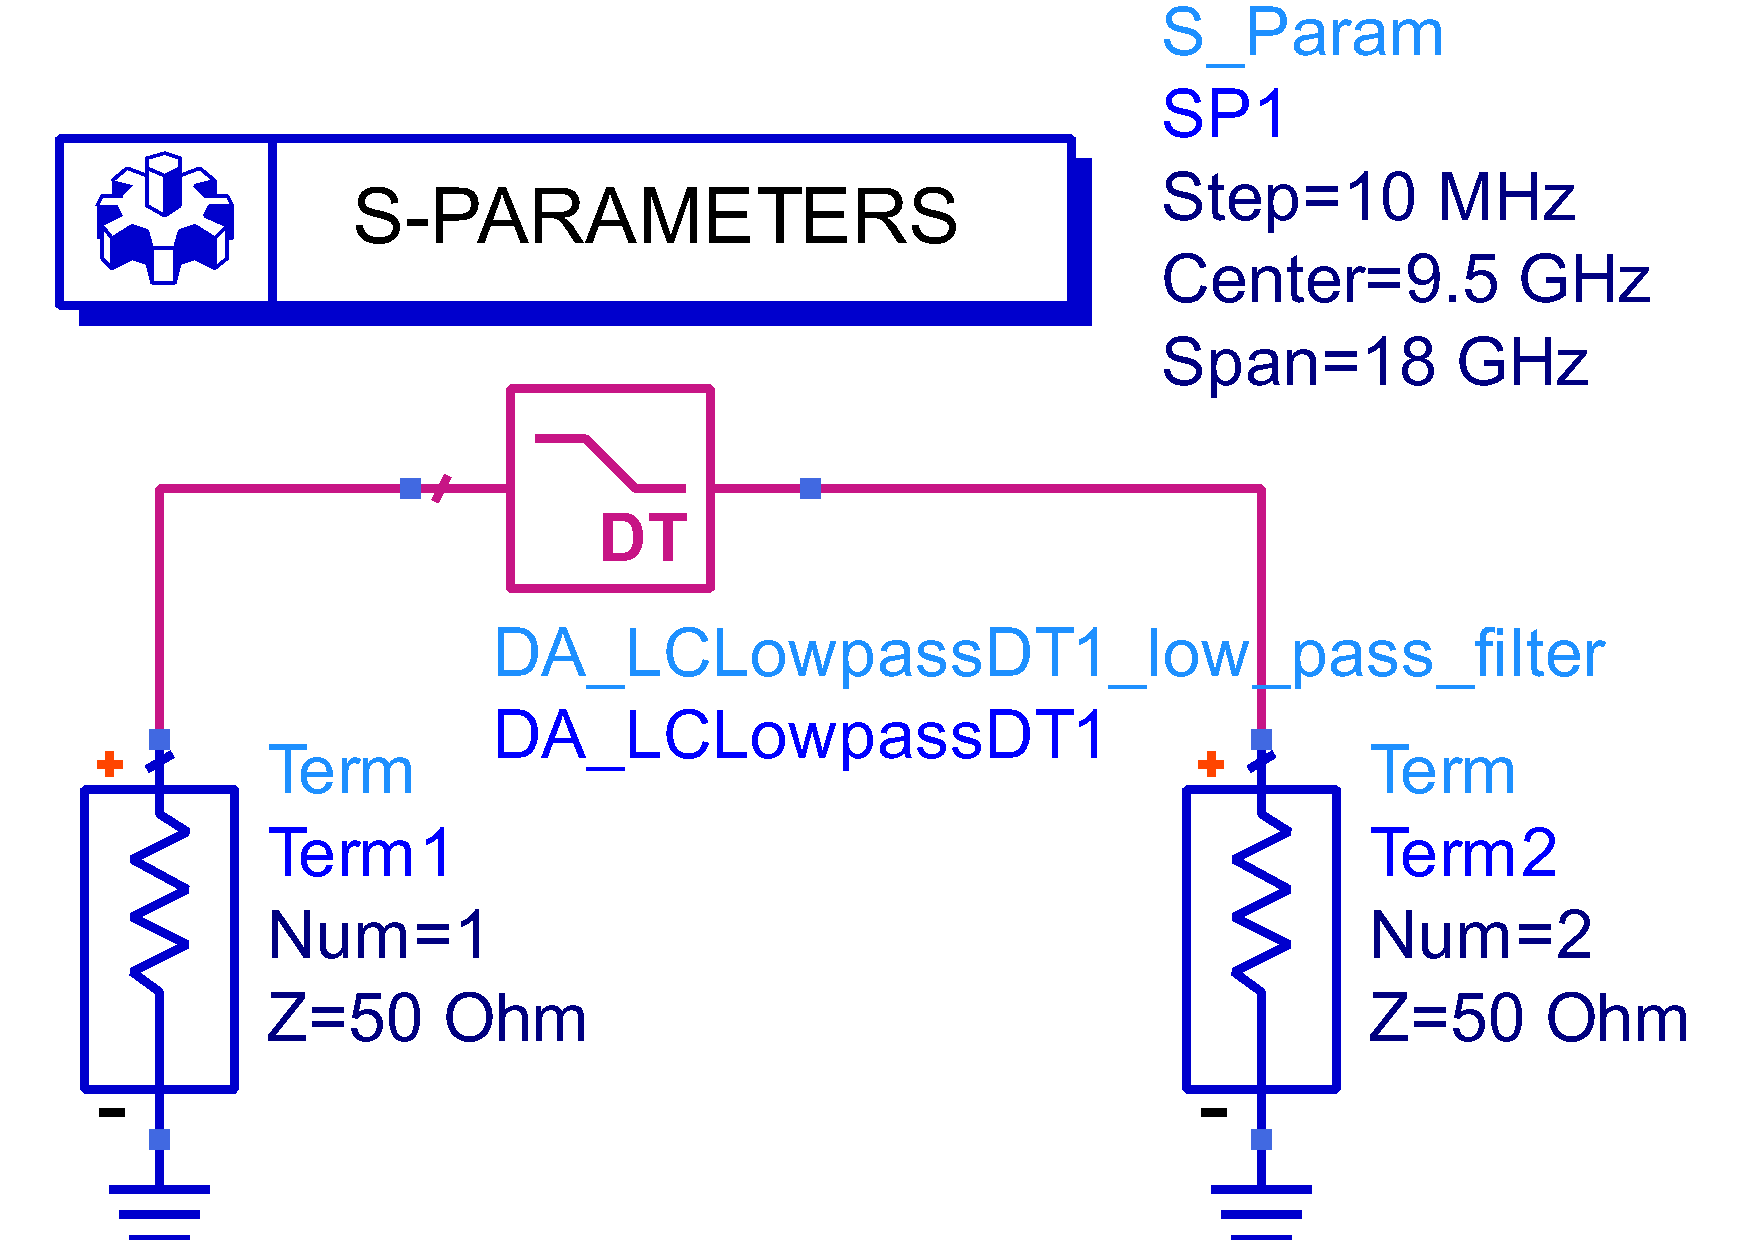
\includegraphics[width=0.6\textwidth]{balanced_mixer_schematic_6.pdf}
    \caption{}%
    \label{fig:balanced_mixer_schematic_6}
\end{figure}

\begin{figure}[!ht]
    \centering
    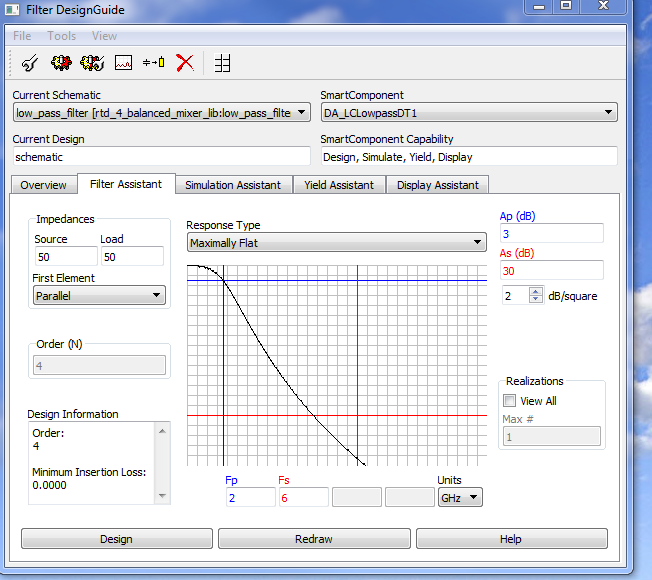
\includegraphics[width=0.6\textwidth]{balanced_mixer_filter_design}
    \caption{}%
    \label{fig:balanced_mixer_filter_design}
\end{figure}

\begin{figure}[!ht]
    \centering
    \begin{subfigure}[b]{0.45\textwidth}
        \centering
        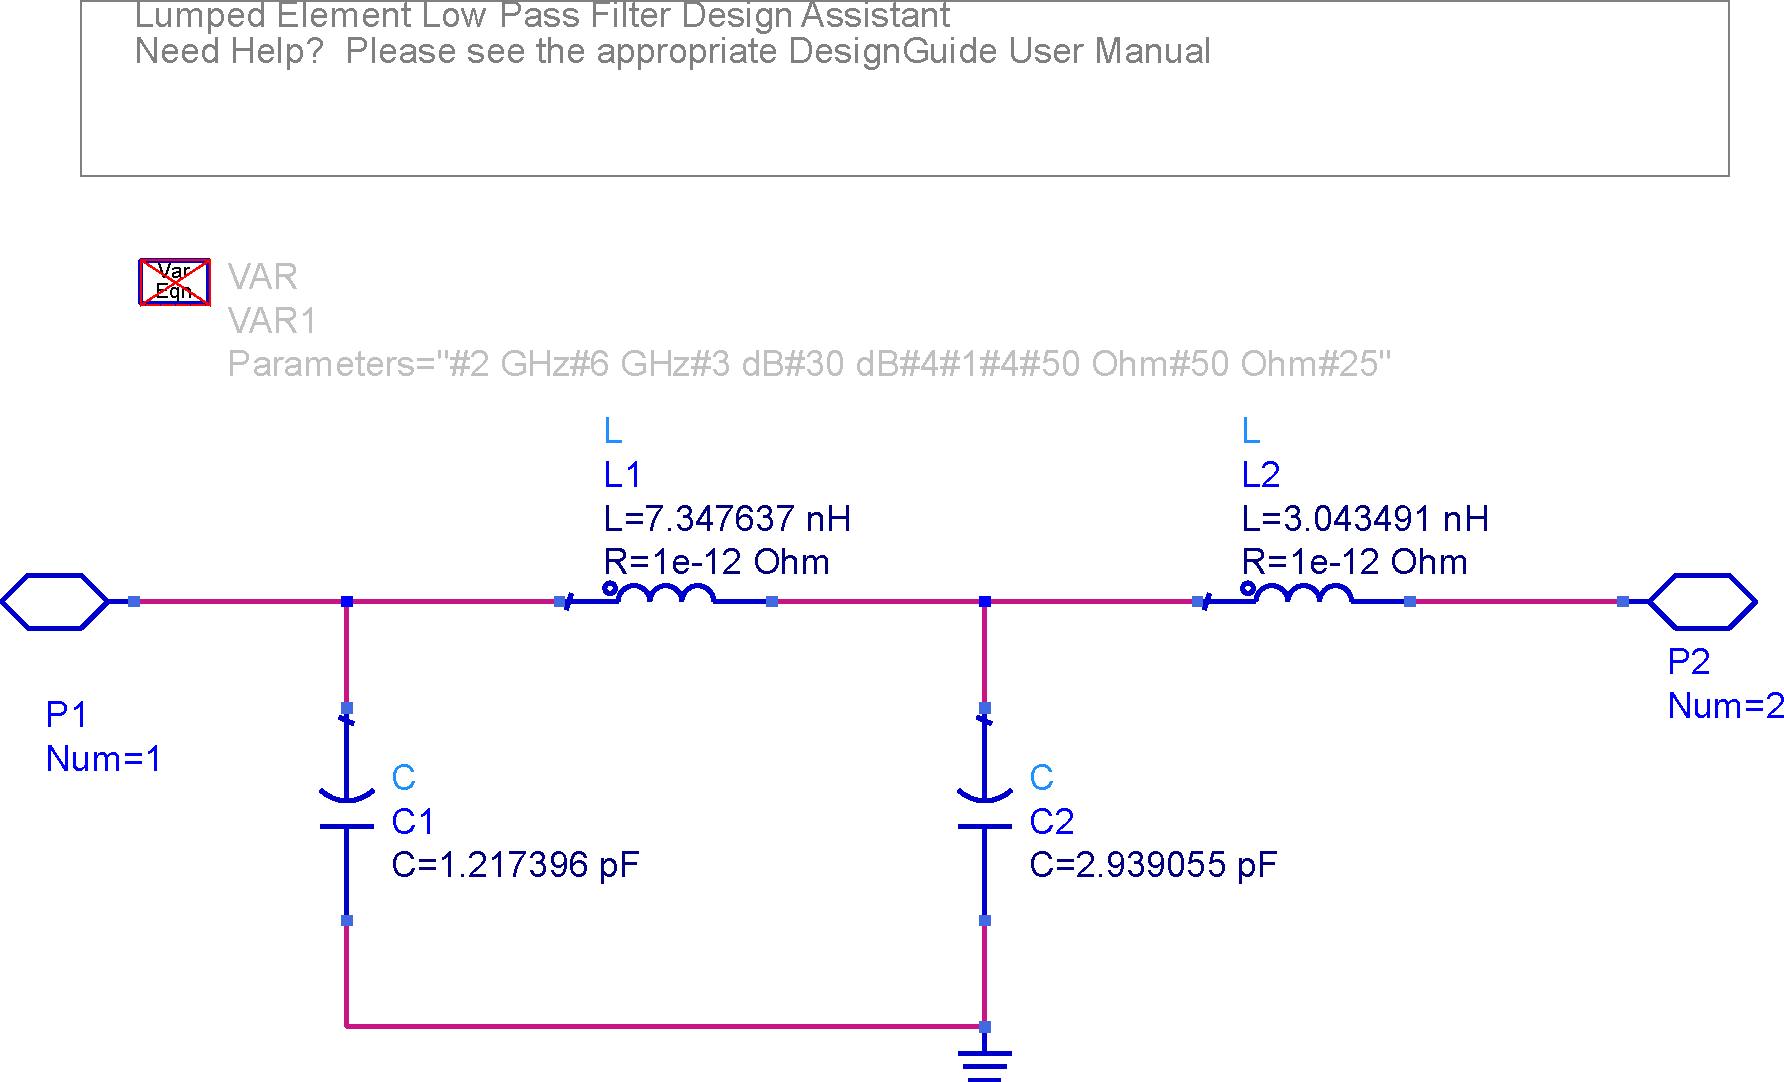
\includegraphics[width=\textwidth]{balanced_mixer_schematic_4.pdf}
        \caption{}%
        \label{fig:balanced_mixer_schematic_4}
    \end{subfigure}
    \hfill
    \begin{subfigure}[b]{0.45\textwidth}
        \centering
        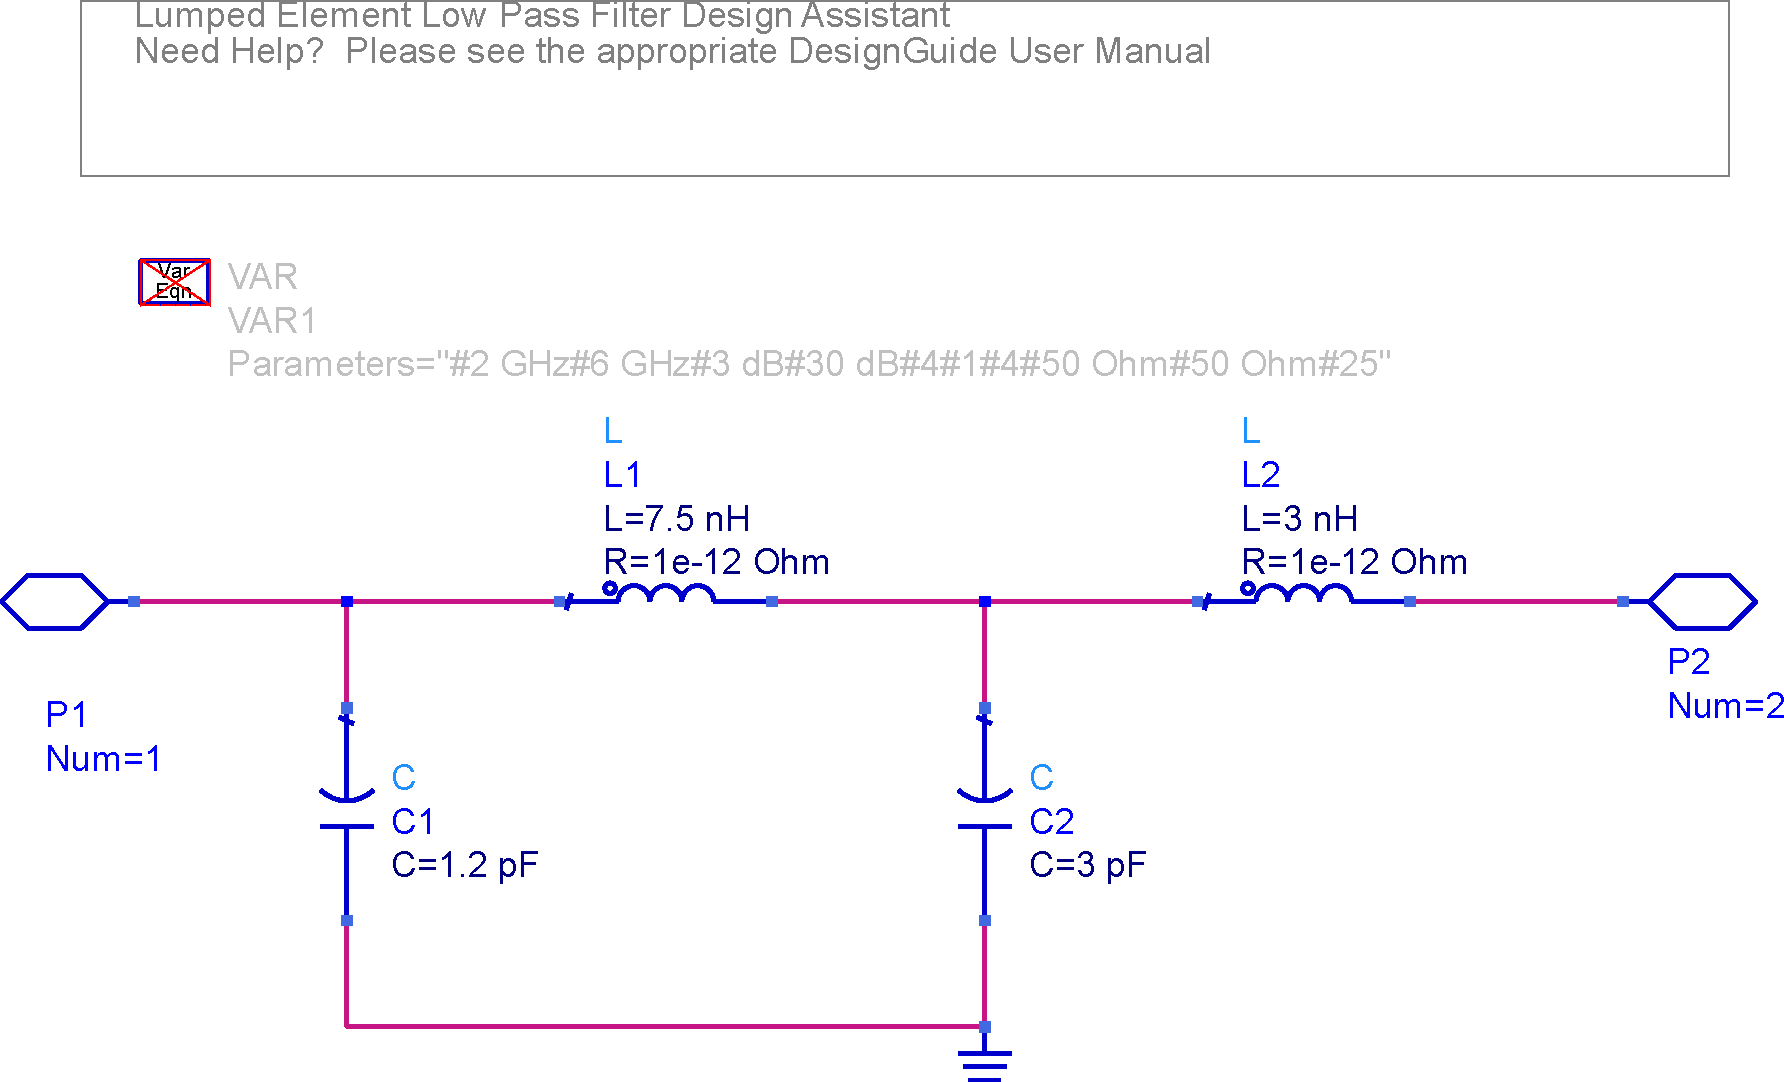
\includegraphics[width=\textwidth]{balanced_mixer_schematic_5.pdf}
        \caption{}%
        \label{fig:balanced_mixer_schematic_5}
    \end{subfigure}
\end{figure}

\begin{figure}[!ht]
    \centering
    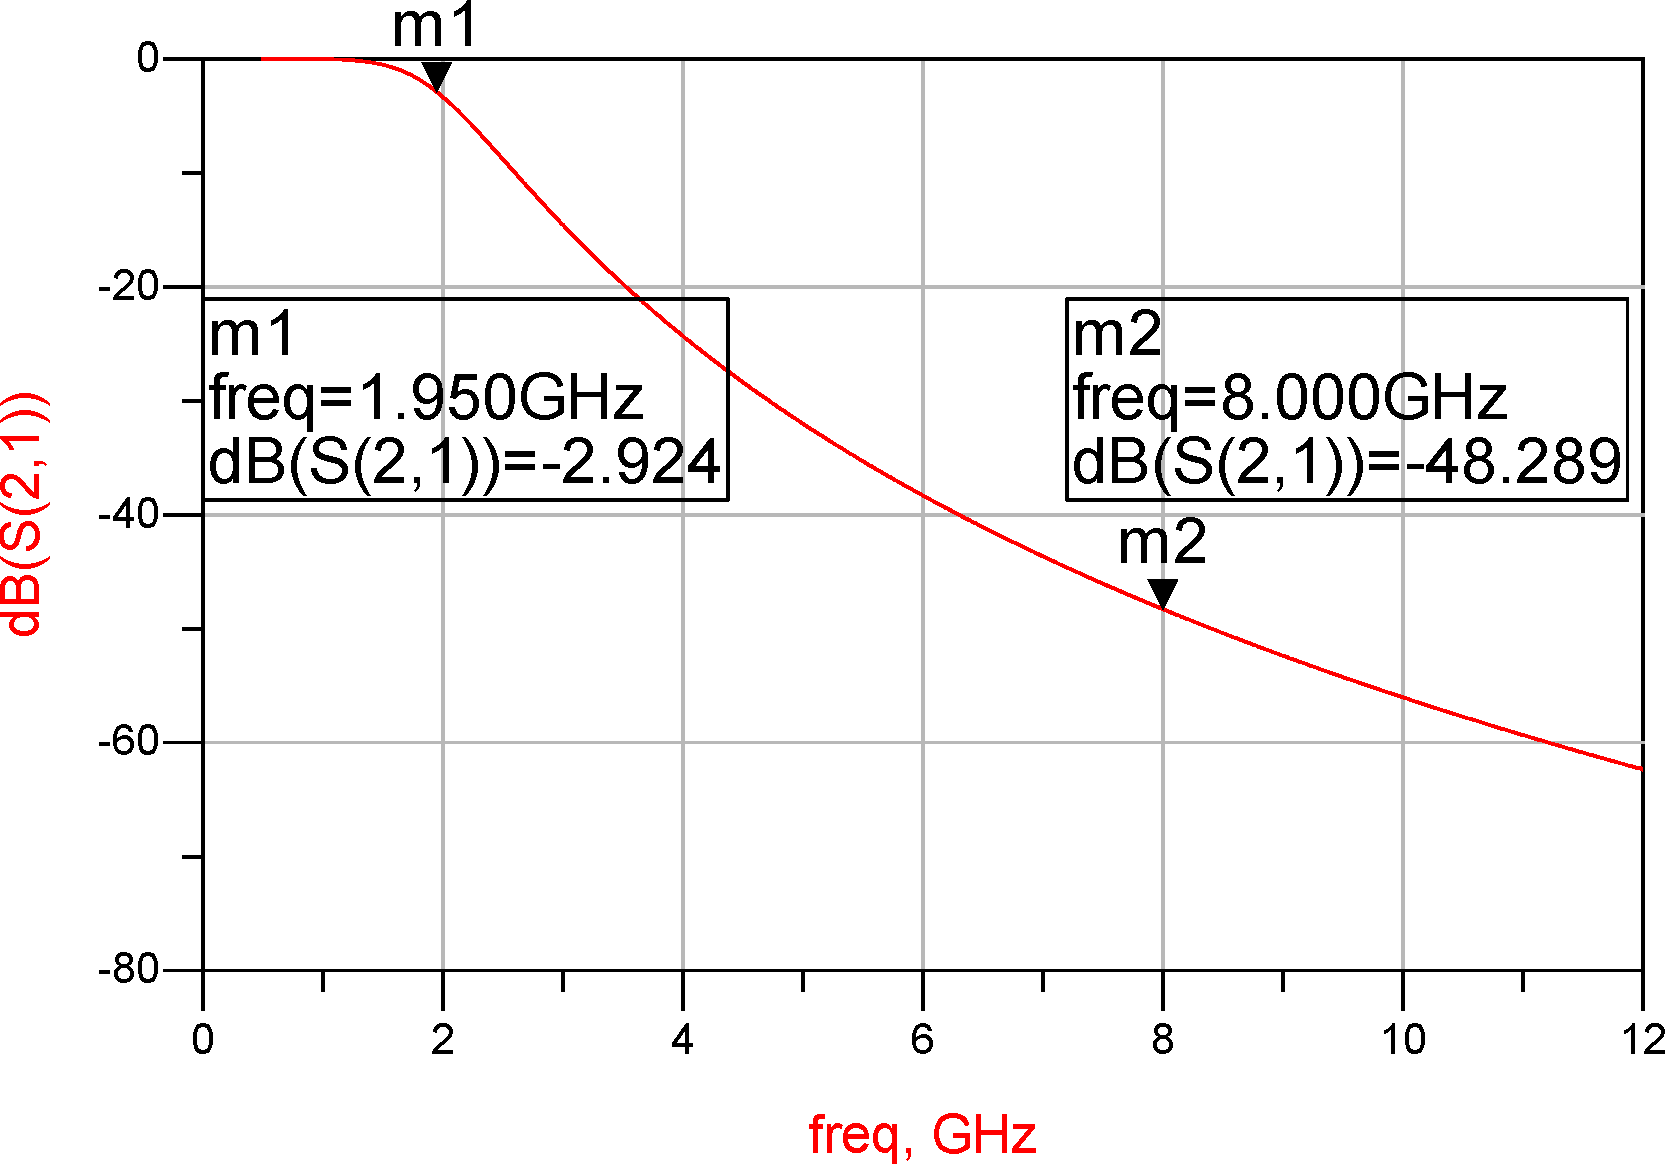
\includegraphics[width=0.6\textwidth]{balanced_mixer_data_4_freq_response.pdf}
    \caption{}%
    \label{fig:balanced_mixer_data_4_freq_response}
\end{figure}

\subsection{Сборка и моделирование смесителя}

Пользуясь синтезированными ранее компонентами соберём балансный смеситель (Рис.~\ref{fig:balanced_mixer_schematic_7}).
Запустим моделирование, после чего на прямоугольном графике выведем семейство линий и выберем среди них наиболее близкую к линейной (Рис.~\ref{fig:balanced_mixer_data_5}).

\begin{figure}[!ht]
    \centering
    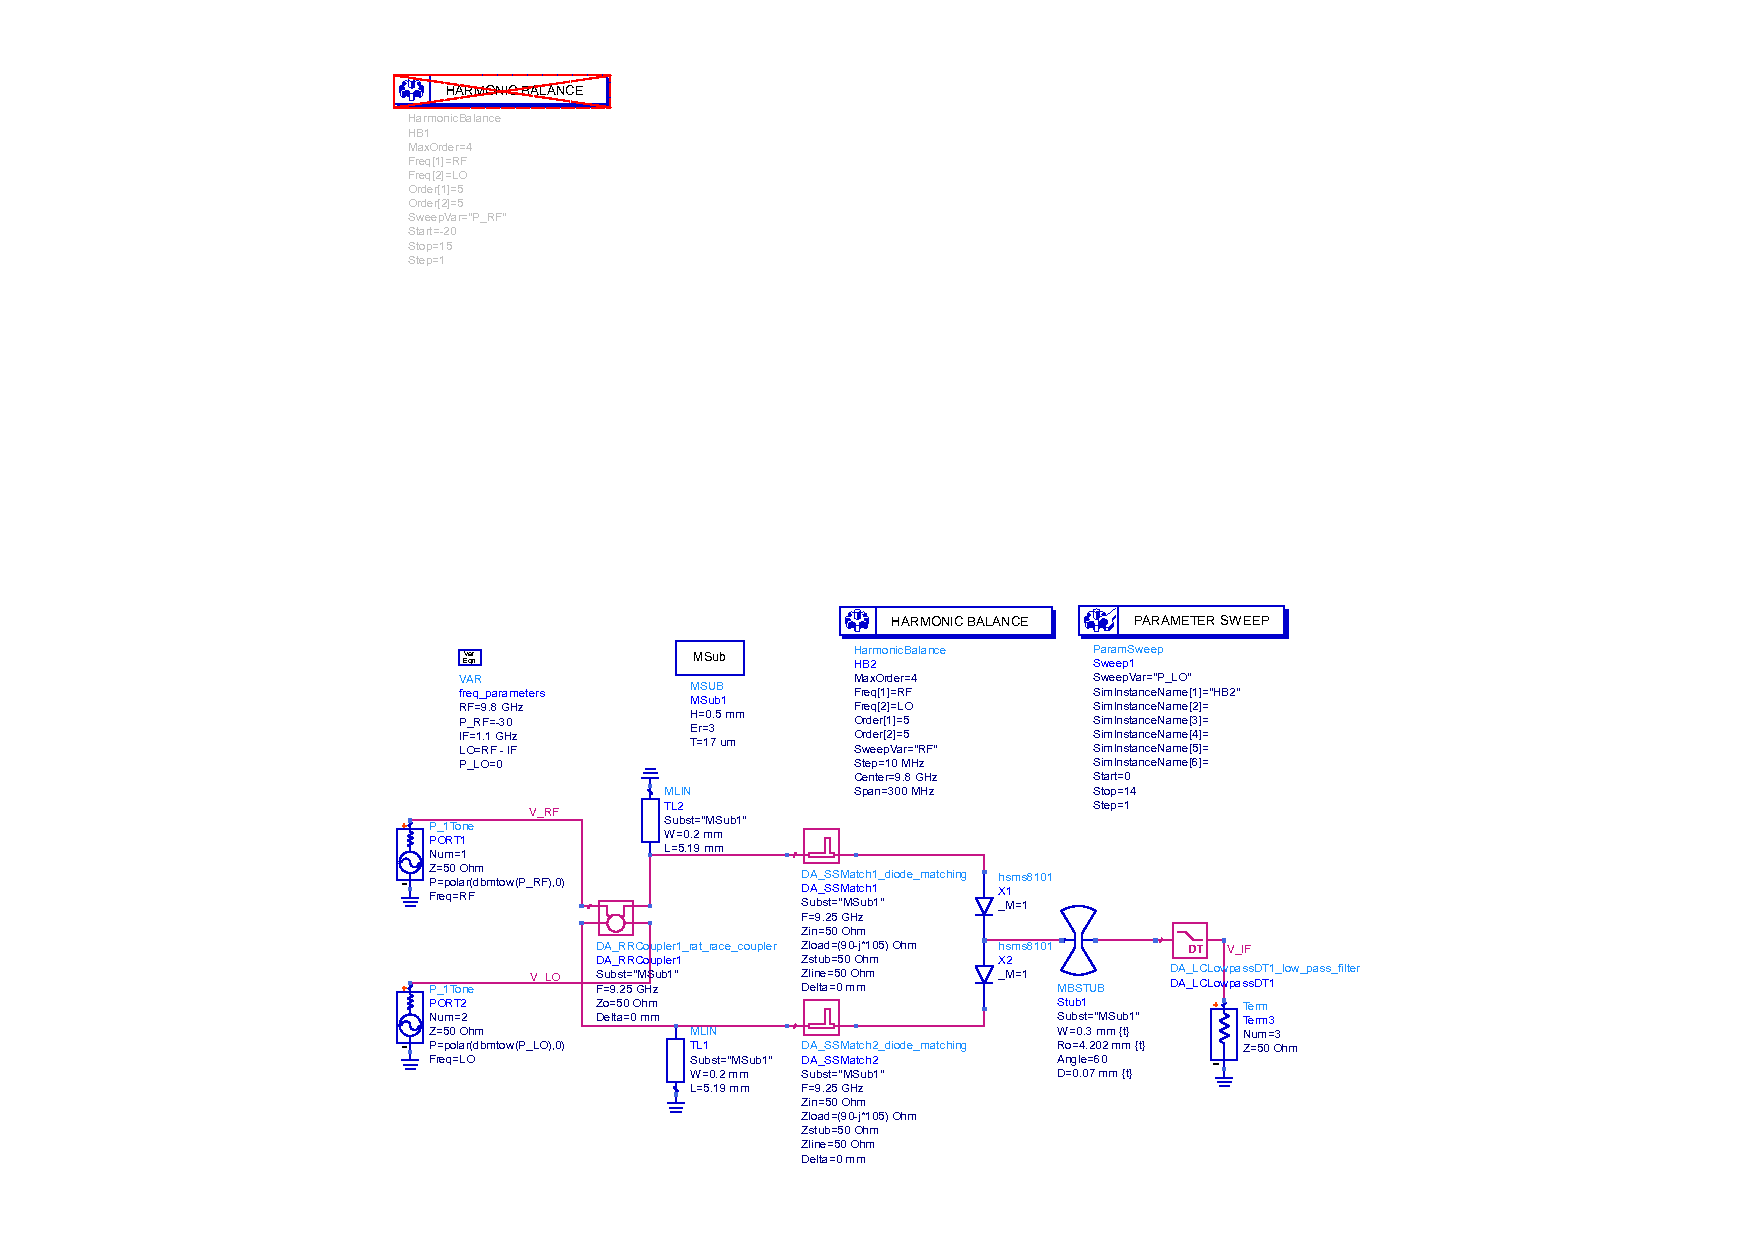
\includegraphics[width=0.6\textwidth]{balanced_mixer_schematic_7.pdf}
    \caption{}%
    \label{fig:balanced_mixer_schematic_7}
\end{figure}

\begin{figure}[!ht]
    \centering
    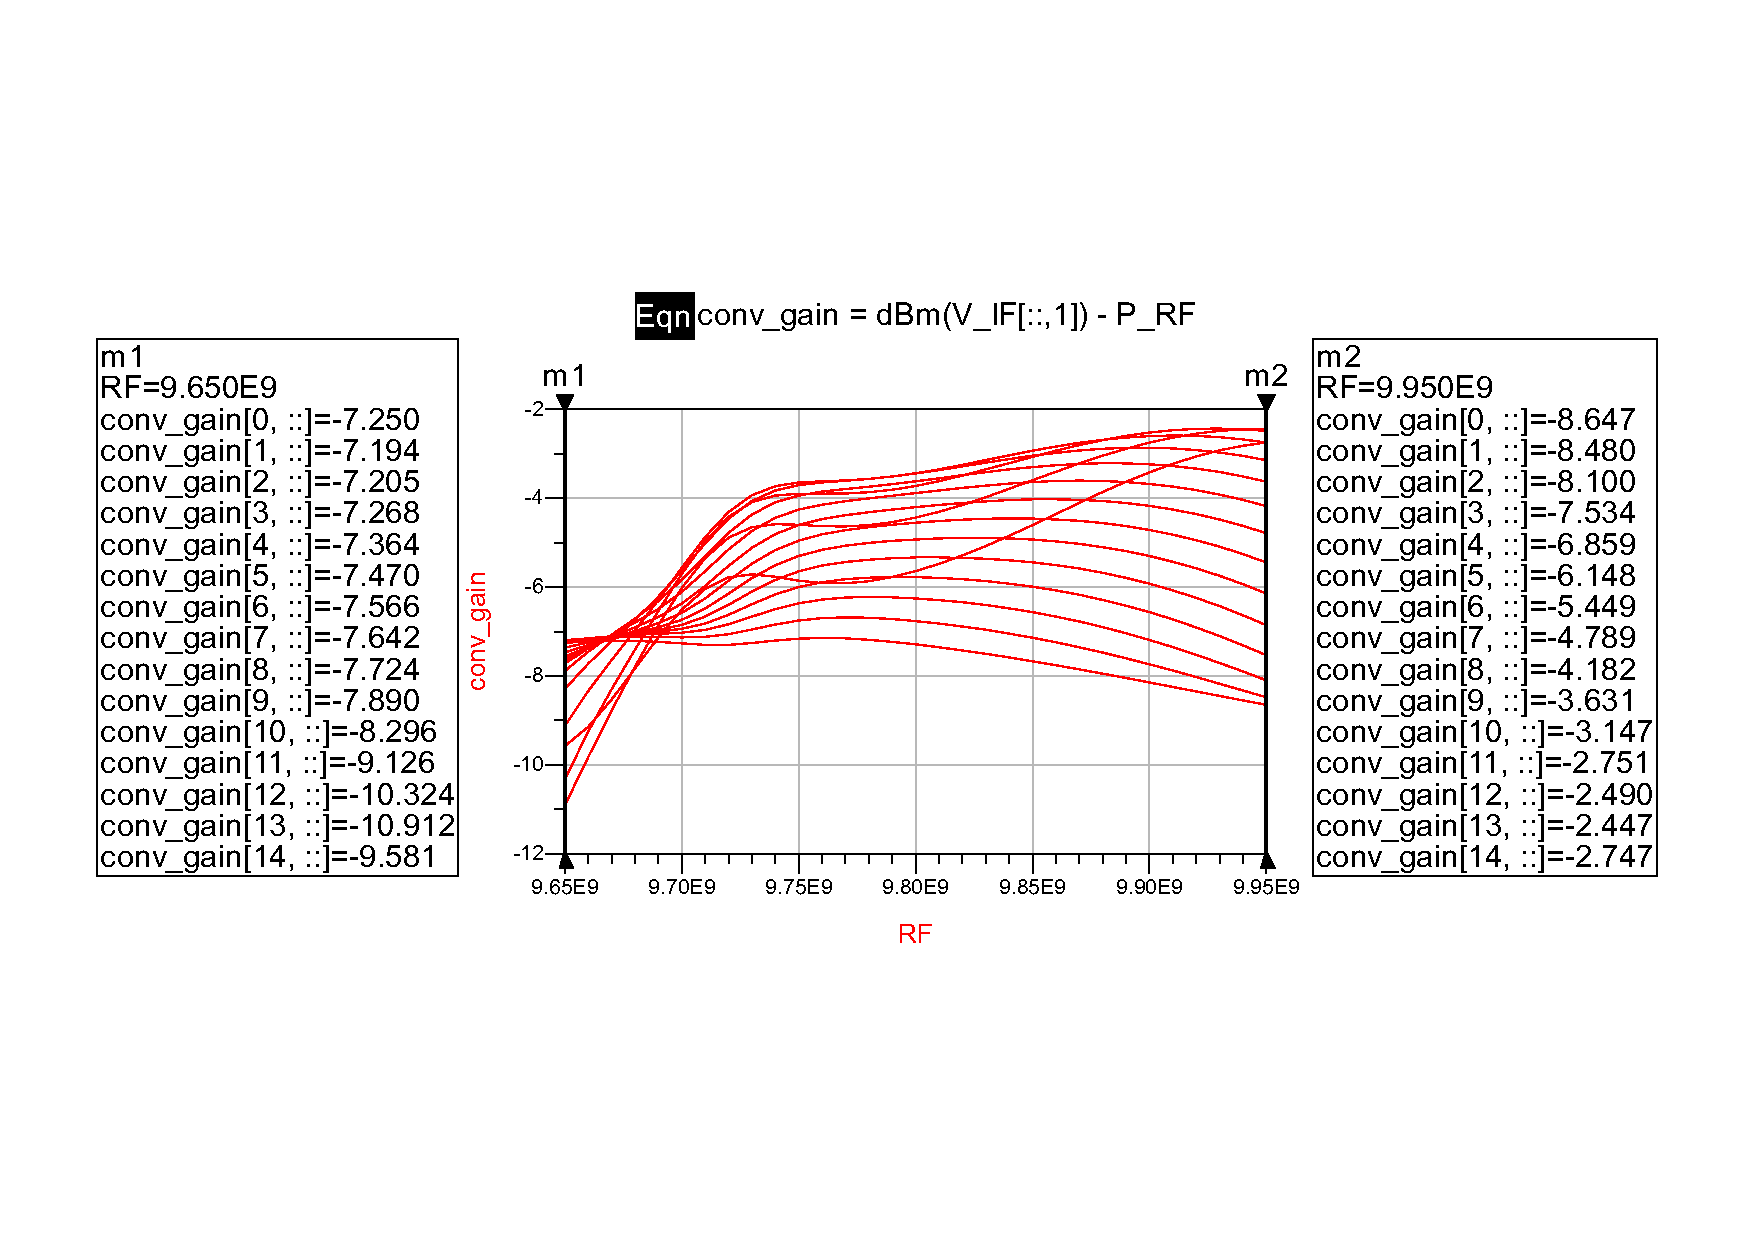
\includegraphics[width=0.6\textwidth]{balanced_mixer_data_5.pdf}
    \caption{}%
    \label{fig:balanced_mixer_data_5}
\end{figure}

Исследуем поведение смесителя при повышении входной мощности.

